\documentclass[a4paper,10pt,landscape,twocolumn]{scrartcl}

%% Settings
\newcommand\problemset{5}
\newcommand\worksession{Tuesday, 26 September 2017}
\newif\ifcomments
\commentsfalse % hide comments
%\commentstrue % show comments

%% Packages
\usepackage[english]{exercises}
\usepackage{wasysym}
\usepackage{graphicx}
\usepackage{hyperref}
\hypersetup{colorlinks=true, urlcolor = blue, linkcolor = blue}
\usepackage{enumitem}

%% Macros
\usepackage{xspace}

\newcommand{\eps}{\varepsilon}
\newcommand{\ket}[1]{|#1\rangle}
\newcommand{\bra}[1]{\langle#1|}
\newcommand{\inp}[2]{\langle{#1}|{#2}\rangle}
\newcommand{\norm}[1]{\parallel\!#1\!\parallel}
\newcommand{\points}[1]{\marginpar{\textbb{#1 p.}}}
\newtheorem{theorem}{Theorem}
\newtheorem{definition}{Definition}
\newtheorem{proposition}{Proposition}
%\newenvironment{proof}{\noindent {\bf Proof }}{{\hfill $\Box$}\\}

\newcommand{\gen}{\ensuremath{\mathsf{Gen}}\xspace}
\newcommand{\enc}{\ensuremath{\mathsf{Enc}}\xspace}
\newcommand{\dec}{\ensuremath{\mathsf{Dec}}\xspace}
\newcommand{\mac}{\ensuremath{\mathsf{Mac}}\xspace}
\newcommand{\vrfy}{\ensuremath{\mathsf{Vrfy}}\xspace}
\newcommand{\negl}{\ensuremath{\mathsf{negl}}\xspace}
\newcommand{\PrivK}{\ensuremath{\mathsf{PrivK}}\xspace}
\newcommand{\eav}{\ensuremath{\mathsf{eav}}\xspace}

\newcommand{\Z}{\ensuremath{\mathbb{Z}}}
\newcommand{\R}{\ensuremath{\mathbb{R}}}
\newcommand{\N}{\ensuremath{\mathbb{N}}}


\newcommand\floor[1]{\lfloor#1\rfloor}
\newcommand\ceil[1]{\lceil#1\rceil}

% \newcommand{\comment}[1]{{\sf [#1]}\marginpar[\hfill !!!]{!!!}}
\newcommand{\chris}[1]{\comment{\color{blue}Chris: #1}}
\newcommand{\jan}[1]{\comment{\color{magenta}Jan: #1}}


\begin{document}

\problems


{\sffamily\noindent
We will work on the following exercises together during the work sessions on \worksession.

You are strongly encouraged to work together on the exercises, including the homework. You do not have to hand in solutions to these problem sets.}



\begin{exercise}[not PRFs]
Let us assume that $k$ and $x$ are $n$-bit strings. For all of the following constructions, explain why they are not PRFs. Give an explicit description of an efficient attacker that distinguishes the given function from a uniform function $f \in \mathsf{Func}_n$.

\begin{subex}
Let $F_k(x)$ output $k$.
\end{subex}

\begin{subex}
Let $F_k(x)$ output $x$.
\end{subex}

\begin{subex}
Let $F_k(x)$ output $x \oplus k$.
\end{subex}

\end{exercise}

\begin{exercise}[Basic properties of PRFs]
The set of all functions from $n$ bits to $\ell$ bits is denoted by
\[ \mathsf{Func}_{n,\ell} := \big\{f:\{0,1\}^n \rightarrow \{0,1\}^{\ell} \big\} \, .
\]
Note that with this definition, we have that $\mathsf{Func}_n$ as defined on page 77 of [KL] is equal to $\mathsf{Func}_{n,n}$.

Let $F:\{0,1\}^n \times \{0,1\}^n \rightarrow \{0,1\}^\ell$ be a pseudorandom function.

\begin{subex}
How many functions are there in $\mathsf{Func}_{n,\ell}$?
\end{subex}

\begin{subex}
How many functions $F_k:\{0,1\}^n \rightarrow \{0,1\}^\ell$ are there if you vary $k$?
\end{subex}

\begin{subex}
What is the fraction of functions $F_k$ among all functions in $\mathsf{Func_{n,\ell}}$?
\end{subex}

\end{exercise}


\begin{exercise}[Exercise~3.14 from $\text{[KL]}$ ]
Argue that if $F$ is a length-preserving pseudorandom function, then
$G(s) := F_s(1)\Vert F_s(2)\Vert \cdots \Vert F_s(\ell)$ is a pseudorandom generator with expansion factor $\ell \cdot n$.
\end{exercise}


\begin{figure}[h]
\center
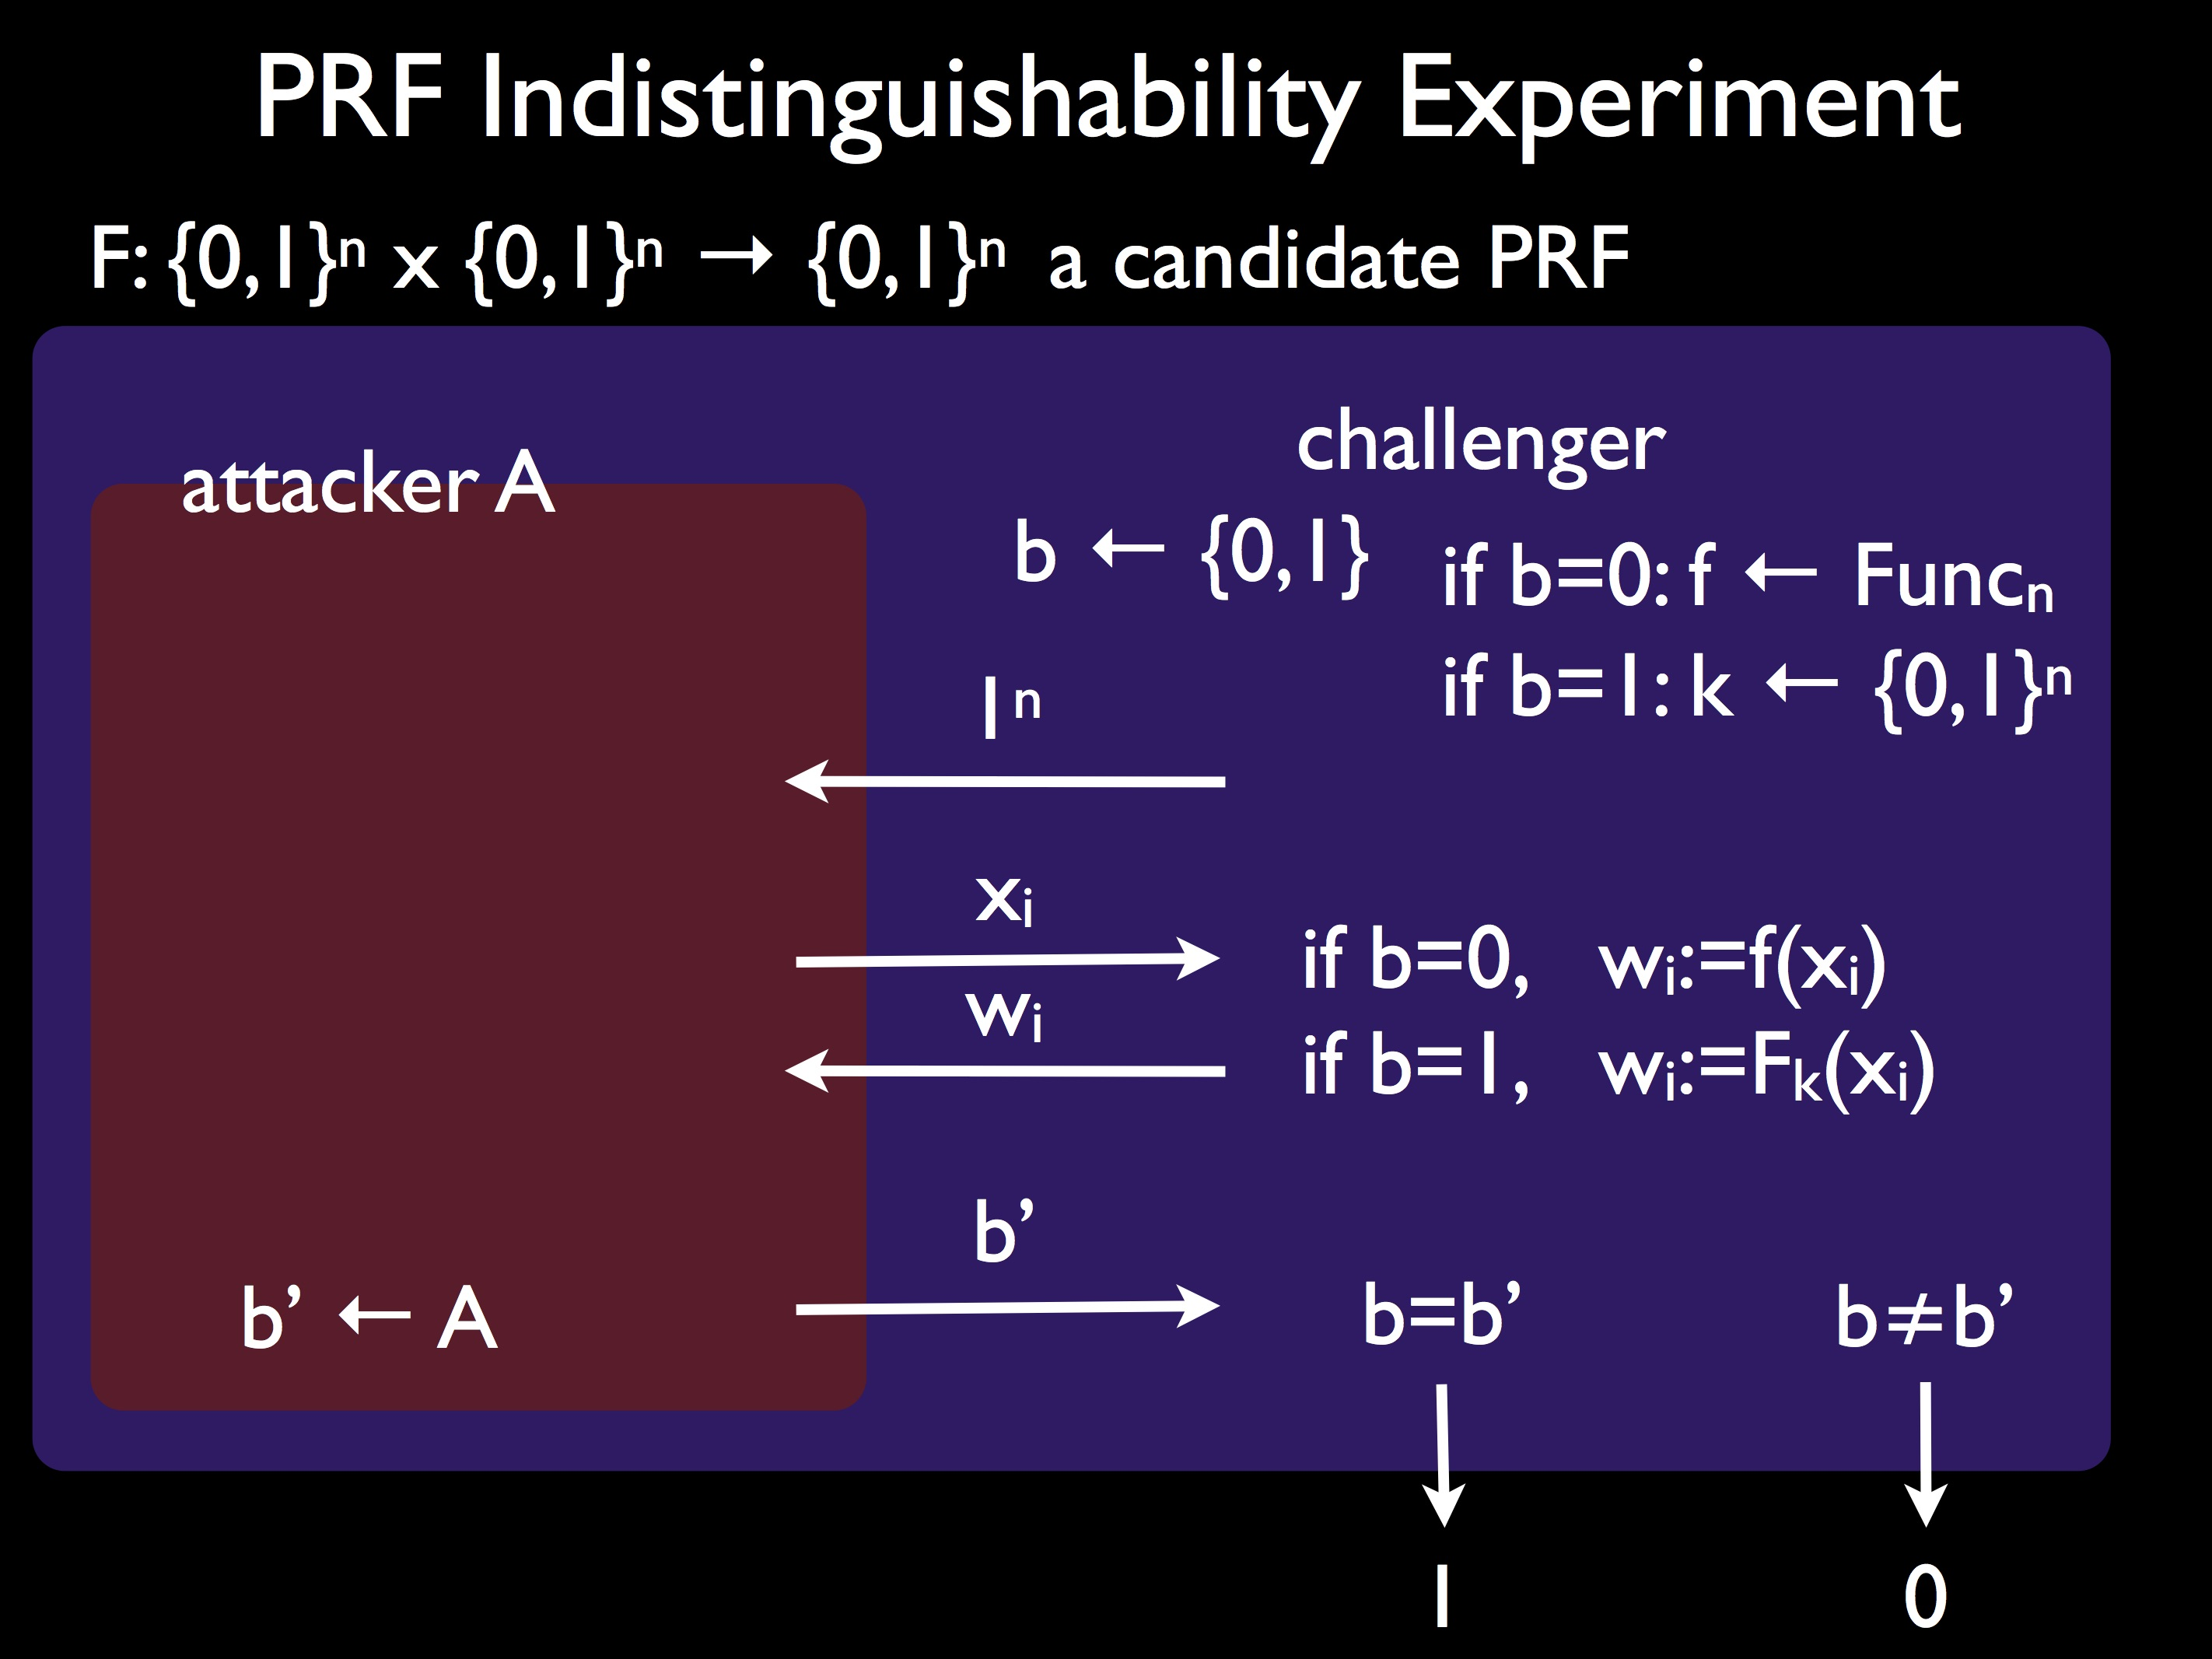
\includegraphics[width=8cm]{PRFExperiment.jpg}
\caption{The $\mathsf{PRF}_{\mathcal{A},F}(n)$ experiment \label{fig}}
\end{figure}

\begin{exercise}[Exercise~3.12]
Let $F$ be a keyed function and consider the following experiment:

\textbf{The PRF indistinguishability experiment $\mathsf{PRF}_{\mathcal{A},F}(n)$:}, see also Figure~\ref{fig}:
\textit{
\begin{enumerate}
\item A uniform bit $b \in \{0, 1\}$ is chosen. If $b = 1$ then choose
uniform $k\in \{0, 1\}^n$ .
\item $\mathcal{A}$ is given $1^n$ for input. If $b = 0$ then $\mathcal{A}$ is given access to
a uniform function $f \in \mathsf{Func}_n$ . If $b = 1$ then $\mathcal{A}$ is instead
given access to $F_k(\cdot)$.
\item $\mathcal{A}$ outputs a bit $b'$.
\item The output of the experiment is defined to be 1 if $b' = b$,
and 0 otherwise.
\end{enumerate}
}

Define pseudorandom functions using this experiment, and prove that
your definition is equivalent to Definition 3.25.
\end{exercise}


\begin{bonusexercise}[Exercise~3.9 from  $\text{[KL]}$ ]
  Prove \emph{unconditionally} the existence of a pseudorandom function $F : \{0,1\}^* \times \{0,1\}^* \to \{0,1\}^*$ with $\ell_{key}(n)=n$ and $\ell_{in}(n)=O(\log n)$.

  \textbf{Hint:} Implement a uniform function with logarithmic input length.
\end{bonusexercise}



\begin{bonusexercise}[Exercise~3.16 from $\text{[KL]}$ ]
  Prove Proposition 3.27:
  \textit{
If $F$ is a pseudorandom permutation and additionally $\ell_{in}(n) \geq n$, then $F$ is also a pseudorandom function.
  }
  
\textbf{Hint:} Use the results of Appendix A.4.
\end{bonusexercise}

\end{document}
